% !TEX TS-program = pdflatex
% !TEX encoding = UTF-8 Unicode

% This is a simple template for a LaTeX document using the "article" class.
% See "book", "report", "letter" for other types of document.

\documentclass[10pt,a4paper]{article}
\newcommand\BK{Benjamin Kowarsch}
\newcommand\RS{Richard J. Sutcliffe}

%\usepackage[utf8]{inputenc} % set input encoding (not needed with XeLaTeX)

%%% Examples of Article customizations
% These packages are optional.
% See the LaTeX Companion or other references for full information.

%%% PAGE DIMENSIONS
\usepackage[top=2.4cm, bottom=2.4cm]{geometry} % to change the page dimensions
\geometry{a4paper} % or letterpaper (US) or a5paper or....
%\geometry{margin=2in} % for example, change the margins to 2 inches all round
%\geometry{landscape} % set up the page for landscape
% read geometry.pdf for detailed page layout information

%\usepackage{graphicx} % support the \includegraphics command and options
%\usepackage[parfill]{parskip} % empty line instead of indent starts paragraph

%%% PACKAGES
\usepackage{enumitem} % for better formatting in item lists
\usepackage{listings} % for better formatting of source code
\usepackage{xcolor} % for grey comments within source code
\usepackage{url} % to position tilde at correct height
\usepackage{graphicx}
%\usepackage{auto-pst-pdf}
%\usepackage{booktabs} % for much better looking tables
%\usepackage{array} % for better arrays (eg matrices) in maths
%\usepackage{paralist} % custom lists (eg. enumerate/itemize, etc.)
%\usepackage{verbatim} % commenting out blocks of text & for better verbatim
%\usepackage{subfig} % include more than one captioned figure/table in a float
% These packages are incorporated in the memoir class to one degree or another.

%%% FONTS
\usepackage{courier}
\usepackage{lmodern}
\makeatletter
\newcommand{\verbatimfont}[1]{\def\verbatim@font{#1}}
\makeatother

%%% HEADERS & FOOTERS
\usepackage{fancyhdr} % This should be set AFTER setting up the page geometry
\pagestyle{fancy} % options: empty , plain , fancy
\fancyhf{}
\lhead{\Title}
\rhead{\thepage}
\cfoot{\small\textsf{\color{gray}Copyright \textcopyright\hspace{0pt} 2018
\BK\hspace{0pt} and \RS\hspace{0pt} -- This draft is for peer review only!}}
% replace with `reproduction permitted for non-commercial use' in final doc

%\renewcommand{\headrulewidth}{0pt} % customise the layout...
%\lhead{}\chead{}\rhead{}
%\lfoot{}\cfoot{\thepage}\rfoot{}

%%% SECTION TITLE APPEARANCE
%\usepackage{sectsty}
%\allsectionsfont{\sffamily\mdseries\upshape} % (see fntguide.pdf)
% (This matches ConTeXt defaults)

%%% ToC (table of contents) APPEARANCE
%\usepackage[nottoc,notlof,notlot]{tocbibind} % Put bibliography in ToC
%\usepackage[titles,subfigure]{tocloft} % Alter style of Table of Contents
%\renewcommand{\cftsecfont}{\rmfamily\mdseries\upshape}
%\renewcommand{\cftsecpagefont}{\rmfamily\mdseries\upshape} % No bold!

\renewcommand{\emph}[1]{\textbf{\textit{#1}}}

\lstdefinestyle{algol}{
  language=[60]Algol,
  frame=none,
  basicstyle=\fontfamily{pcr}\selectfont,
  keywordstyle=\textbf,
  commentstyle=\italicgray
}

\lstdefinestyle{C}{
  language=[ANSI]C,
  frame=none,
  basicstyle=\fontfamily{pcr}\selectfont,
  keywordstyle=\textbf,
  commentstyle=\italicgray
}

\lstdefinestyle{modula2}{
  language=Modula-2,
  frame=none,
  morekeywords={CAPACITY, INDETERMINATE, NEW, TO},
  basicstyle=\fontfamily{pcr}\selectfont,
  keywordstyle=\textbf,
  commentstyle=\italicgray
}

\lstdefinestyle{pascal}{
  language=Pascal,
  frame=none,
  basicstyle=\fontfamily{pcr}\selectfont,
  keywordstyle=\textbf,
  commentstyle=\italicgray
}

\newcommand\boldgray[1]{\textcolor{gray}{\textbf{#1}}}
\newcommand\italicgray[1]{\textcolor{gray}{\textit{#1}}}
\newcommand\middledots{\textperiodcentered\textperiodcentered\textperiodcentered}
\newcommand\sourcecaption[1]{\noindent\normalfont\small\textsf{#1}}

%%% Glossary
\usepackage[automake, nonumberlist, style=altlist]{glossaries}
\makeglossaries
\newglossaryentry{API}{
  name=API,
  description={Application programming interface}
}
\newglossaryentry{capacity field}{
  name=capacity field,
  description={a field of an \gls{indeterminate type} to
  hold the allocation size of an \gls{indeterminate field}}
}
\newglossaryentry{indeterminate field}{
  name=indeterminate field,
  description={a field of an \gls{indeterminate type} whose size
  is determined during allocation at runtime}
}
\newglossaryentry{indeterminate type}{
  name=indeterminate type,
  description={a compound type with at least a \gls{capacity field} and
  an \gls{indeterminate field}}
}

\usepackage{pifont}
\renewcommand{\glstextformat}[1]{\textit{#1}}


%%% END Article customizations


%%% D O C U M E N T   S T A R T S   H E R E

% *****************************************************************************
% T  i  t  l  e
% *****************************************************************************
\title{Type Safe Indeterminate Records}
\author{\BK\hspace{0pt} and \RS, Modula-2 Software Foundation}
\date{\small{October 2018 (Draft 3)}}
\makeatletter
\let\Title\@title
\makeatother
\makeatletter
\let\Author\@author
\makeatother


\begin{document}
\verbatimfont{\small\fontfamily{lmtt}\selectfont}
\maketitle

% *****************************************************************************
% A  b  s  t  r  a  c  t
% *****************************************************************************
\begin{abstract}
The C language has long provided a facility to declare a \verb|struct| with
a variable length array field whose size is determined when an instance
of the \verb|struct| is allocated at runtime. Such a facility is a useful
building block for the construction of opaque abstract data types. The classic
Modula-2 language \cite{Wirth88, ISO96} lacks such a facility. In this paper we
show how a type safe equivalent can be added to a Modula-2 implementation as a
language extension.
\end{abstract}


% *****************************************************************************
% I  n  t  r  o  d  u  c  t  i  o  n
% *****************************************************************************
\section{Introduction}

In the 1960s it was common for arrays and buffers to be statically allocated
at compile time. Upper and lower bounds of arrays and buffers were hardcoded.

\paragraph{\sourcecaption{Array Declaration in Algol-60 \cite{Backus60}}}~

\lstset{style=algol}
\begin{lstlisting}
integer array a[0:255];
\end{lstlisting}~

\noindent This turned out to be cumbersome when the array bounds needed to
be changed. By the 1970s it was common to provide a facility to define
constants and use them within array declarations.

\paragraph{\sourcecaption{Array Declaration in Pascal \cite{JW74}}}~

\lstset{style=pascal}
\begin{lstlisting}
const MaxIndex = 255;
var a : array [0..MaxIndex] of integer;
\end{lstlisting}~

\noindent Whilst array bounds could now easily be changed in a single
location, the program needed to be recompiled after any such change.
By the 1980s it was common to exploit a loophole in the C~language
by which the size of an array could be set to zero.

\paragraph{\sourcecaption{Zero Length Array Declaration in
ANSI-C \cite{ANSI-C}}}~

\lstset{style=C}
\begin{lstlisting}
typedef struct {
  unsigned size;
  unsigned length;
  int buffer[0]; /* pretend an array of size 0 */
} vla_t;
\end{lstlisting}~

\noindent Since C does not do any array bounds checking it is possible
to allocate an array of a different size than that given in its declaration
and thereby gain the facility of a variable length array whose size is
determined during allocation at runtime.

\paragraph{\sourcecaption{Variable Length Array Allocator in ANSI-C}}~

\lstset{style=C}
\begin{lstlisting}
vla_t *new_array ( unsigned size ) {
  vla_t *array = malloc(sizeof(unsigned)+size*sizeof(int));
  if (array != NULL) {
    array->size = size;
  }; /* if */
  return array;
}; /* new_array */
\end{lstlisting}

\noindent The ISO-C working group then incorporated this practice into the
ISO-C standard of 1990 by permitting the size parameter in an array declaration
to be omitted when its size is intended to be determined at runtime.

\paragraph{\sourcecaption{Variable Length Array Declaration in
ISO-C90 \cite{ISO-C}}}~

\lstset{style=C}
\begin{lstlisting}
typedef struct {
  unsigned size;
  unsigned length;
  int buffer[]; /* size to be determined at runtime */
} vla_t;
\end{lstlisting}~

\noindent Unfortunately, this facility is unsafe. There is no requirement 
for any field to store the allocated size, nor any mechanism to ensure that
the field if present stores the actual size, let alone a requirement to
perform bounds checking on the array field against the actual size.\\

\noindent This means plenty of opportunity for error and opens up the software
to buffer overflows with fatal consequences for reliability and security. The 
facility is one of the single most important causes of buffer overflow
exploits.


\paragraph{\sourcecaption{Buffer Overflow in C}}~

\lstset{style=C}
\begin{lstlisting}
vla_t *array = new_array(99); /* allocated buffer size 99 */
array->buffer[100] = 0; /* writing beyond allocated buffer */
\end{lstlisting}~
 
\noindent The ISO-C working group would have done the world a great service
had they put in a little more effort and care to design a safe variable length
array facility for the ISO-C standard.\\

\noindent For a safe facility, all of the following conditions must be met:

\renewcommand{\labelenumi}{(\arabic{enumi})}
\begin{enumerate}[leftmargin=!, labelindent=-0.75em, itemindent=0em]
\item mandatory presence of a \gls{capacity field}
\item exclusive use of an allocation mechanism that takes a size parameter,
allocates an instance of an \gls{indeterminate type} and initializes its
\gls{capacity field} with the allocated size
\item the \gls{capacity field} must be protected from write
access after its initialization
\end{enumerate}

\noindent Condition (1) could be met by requiring the \gls{capacity field}
to be referenced as size parameter in the array declaration of the variable
length array field.

\lstset{style=C}
\begin{lstlisting}
typedef struct {
  unsigned size; /* capacity field */
  unsigned length; /* runtime length field */
  int buffer[size]; /* indeterminate field */
} vla_t; /* indeterminate type */
\end{lstlisting}~

\noindent Condition (2) could be met by introducing a specialized allocator 
function requiring its use.

\lstset{style=C}
\begin{lstlisting}
vla_t *array = valloc(99); /* VLA specific allocator */
\end{lstlisting}~

\noindent Condition (3) could be enforced during static analysis at compile 
time.

\lstset{style=C}
\begin{lstlisting}
array->size = 1000; /* illegal operation, immutable field */
\end{lstlisting}~


\noindent The challenge then lies in defining semantics for compatibility and
copying of entities of an \gls{indeterminate type}. To do so for C would be the
subject  of another paper. In this paper, we will present a complete and type 
safe design of indeterminate record types for Modula-2.

\newpage

% *****************************************************************************
% D  e  s  i  g  n     C  o  n  s  i  d  e  r  a  t  i  o  n  s
% *****************************************************************************
\section{Design Considerations}

\subsection{Simplicity of Syntax}

Ideally, the introduction of additional reserved words should be avoided.
If a new reserved word was to be introduced, it should be short and intuitive.
There should be no more than three consecutive reserved words anywhere in the
grammar.\\

\par\noindent Whilst Modula-2 is relatively verbose when compared to C and its
derivatives, the use of reserved words is rather moderate when compared to
COBOL or PL/1. Most reserved words are short and typically occur sole or in
pairs such as \verb|ARRAY OF|, and in a few cases in sequences of three such as
\verb|POINTER TO RECORD|.  


\subsection{Preservation of LL(1) Properties}

Any new syntax for the declaration of indeterminate types should preserve the
LL(1) properties~\cite{Lewis68} of the Modula-2 grammar.\\

\par\noindent
When extending an existing language, newly introduced facilities should be
designed to follow the general design philosophy of the language if only for
the benefit of consistency. 

Since the introduction of Pascal \cite{JW74} in 1970, all Wirthian languages
have been designed for recursive descent parsing \cite[p.5]{Moessenboeck00}.
That is to say, their grammars have been designed to meet LL(1) constraints.
The benefits are manifold. Not only are recursive descent parsers simpler,
faster and easier to maintain\footnote{citation needed, BK: Moessenboeck
mentions this but a separate reference would be better}, but languages that
have been specifically designed for LL(1) are generally more intuitive and
less error prone to use\footnote{citation needed, BK: Wirth mentions this in
several of his books and papers, but I could not find it}.


\subsection{Prevent Static Allocation}

It should not be possible to statically allocate an instance of an
indeterminate type.\\

\par\noindent The primary purpose of an indeterminate type is to delay the
determination of allocation size from compile time to runtime. This
necessitates dynamic allocation. Static allocation of an instance of an
indeterminate type does not make any sense and should be prevented by
design.

There are two possible approaches: In one approach, the grammar does not
permit any construct to declare a static variable of an indeterminate
type and any such attempt is then rejected during syntax analysis. In the
other approach, the grammar permits the declaration of a static variable
of an indeterminate type and its allocation is then rejected during
semantic analysis. The former approach is preferable because it is more
comprehensible. A human reader can deduce the rules from the grammar alone.
The latter approach potentially violates the principle of least surprise
\cite{Geoffrey87} since the rules cannot be deduced from the grammar.


\subsection{Hiding Internal Structure}

It should not be possible to make the internal structure of an indeterminate
type public. Its declaration should always have to be confined within an
implementation part. It should not be permitted within an interface part.\\

\par\noindent Modula-2 lexically separates interface and implementation into
separate compilation units. A so called definition module constitutes the
public interface, while its counterpart, the implementation module contains
the implementation details which are hidden from any client module.

The ability to incorporate a variable length array field into a compound
type is most useful when it is used as a building block for abstract
data types. In Modula-2, abstract data types are realised through so called
opaque types. An opaque type's name is defined in the definition module of
the library that provides it, and its declaration is hidden in the
corresponding implementation module. Access to the internal data of an
instance of such a type is only available through getter and setter
procedures in the public interface of the type, hence it is opaque.



% *****************************************************************************
% E  v  o  l  u  t  i  o  n     o  f     t  h  e     D  e  s  i  g  n
% *****************************************************************************
\section{Evolution of the Design}

Our very first attempt to design syntax for the declaration of indeterminate
types was a na\"ive adaptation of the \verb|struct| syntax found in C,
incorporating an explicit capacity field into the record declaration. In order
to distinguish ordinary from indeterminate record declarations whilst
preserving the LL(1) property of the grammar, we introduced a new reserved word
\verb|INDETERMINATE| to precede the record declaration. 

\paragraph{\sourcecaption{Indeterminate Record Declaration in Modula-2
-- Version 1}}~

\lstset{style=modula2}
\begin{lstlisting}
TYPE VLA = POINTER TO VLADescriptor;

TYPE VLADescriptor = INDETERMINATE RECORD
  capacity,
  length  : CARDINAL;
+ buffer : ARRAY capacity OF INTEGER
END; (* VLADescriptor *)
\end{lstlisting}~

\par\noindent Two disadvantages are immediately apparent in this design. First,
it requires an additional reserved word possibly conflicting with user-defined
identifiers in existing Modula-2 source text and owing to the need of being
self-explanatory, the chosen reserved word is rather long.

Second and more importantly, the syntax permits the declaration of variables
of the intermediate record descriptor type and thus it does not prevent static
allocation of instances of an indeterminate type during syntax analysis. It
would need to be rejected during semantic analysis.

\paragraph{\sourcecaption{Undesired Static Allocation}}~
\lstset{style=modula2}
\begin{lstlisting}
VAR vla : VLADescriptor; (* this needs to be rejected *)

\end{lstlisting}~

\par\noindent After much experimentation, we resolved both issues by removing
the ability to declare an intermediate record descriptor type, instead
requiring the record descriptor to be incorporated into the pointer type
declaration.

\paragraph{\sourcecaption{Indeterminate Record Declaration in Modula-2
-- Version 2}}~

\lstset{style=modula2}
\begin{lstlisting}
TYPE VLA = POINTER TO RECORD
  capacity,
  length  : CARDINAL;
+ buffer : ARRAY capacity OF INTEGER
END; (* VLA *)
\end{lstlisting}~

\par\noindent We then found that the syntax did not seem to be as intuitive as
it had appeared to us. We had assumed that it would be apparent and obvious
that the \verb|capacity| field stored the value of the actually allocated
capacity of the \verb|buffer| field after allocation at runtime since the
\verb|ARRAY| declaration references it. However, a number of peers to whom we
had sent a preliminary specification for review did not make that connection.

Furthermore, since the indeterminate type declaration is to be hidden in an
implementation module, the \verb|capacity| field would not be accessible from
a client module. For every indeterminate type, a user-defined getter function
would need to be written and made available in the interface.

\paragraph{\sourcecaption{User Defined Capacity Function}}~

\lstset{style=modula2}
\begin{lstlisting}
PROCEDURE capacity ( vla : VLA ) : CARDINAL;
BEGIN
  IF vla = NIL THEN
    RETURN 0
  ELSE
    RETURN vla^.capacity
  END (* IF *)
END capacity;
\end{lstlisting}

\par\noindent This seemed like unnecessary boilerplate. Eventually, we arrived
at the insight that we could dispense with an explicit capacity field
altogether by making it implicit and hidden.

\paragraph{\sourcecaption{Indeterminate Record Declaration in Modula-2
-- Final Version}}~

\lstset{style=modula2}
\begin{lstlisting}
TYPE VLA = POINTER TO RECORD
(* hidden capacity : CARDINAL; *)
  length : CARDINAL;
+ buffer : ARRAY OF INTEGER
END; (* VLA *)
\end{lstlisting}~

\par\noindent The language processor implicitly inserts a hidden capacity
field into any indeterminate record and \verb|NEW| automatically initializes
the field during allocation at runtime.

\paragraph{\sourcecaption{Allocating an Instance with a buffer Capacity of 1000}}~

\lstset{style=modula2}
\begin{lstlisting}
NEW vla OF 1000; (* Modula-2 R10 *)
NEW(vla, 1000); (* Classic and ISO Modula-2 *)
\end{lstlisting}~

\par\noindent For the purpose of obtaining the capacity of an instance of an
indeterminate type, we introduced a new pervasive function
\verb|CAPACITY()|. Alternatively, in classic Modula-2 and ISO Modula-2
pervasive function \verb|HIGH()| could be extended for this purpose.

\paragraph{\sourcecaption{Querying the Capacity}}~

\lstset{style=modula2}
\begin{lstlisting}
n := CAPACITY(vla); (* Modula-2 R10 *)
n := HIGH(vla); (* Classic and ISO Modula-2 *)
\end{lstlisting}~


\par\noindent Making the capacity field implicit and hidden also has the
advantage that a language processor does not need to handle and reject
attempts to write to the field witin the implementation module in which
it would otherwise be visible.

\paragraph{\sourcecaption{Invisibility of the Capacity Field}}~

\lstset{style=modula2}
\begin{lstlisting}
vla^.capacity := 0; (* undefined field: capacity *)
\end{lstlisting}~


\noindent TO DO:

\renewcommand{\labelenumi}{(\arabic{enumi})}
\begin{enumerate}[leftmargin=!, labelindent=-0.75em, itemindent=0em]
\item copy and adapt specification from M2R10 (BSK) wiki at Github
\item show use case in C and ISO Modula-2 (using address arithmentic)
\item show same use case in Modula-2 (using indeterminate type facility)
\end{enumerate}

\noindent to be continued ...\\

\newpage

\section{Syntax}

\paragraph{\sourcecaption{Type Declaration}}~

\noindent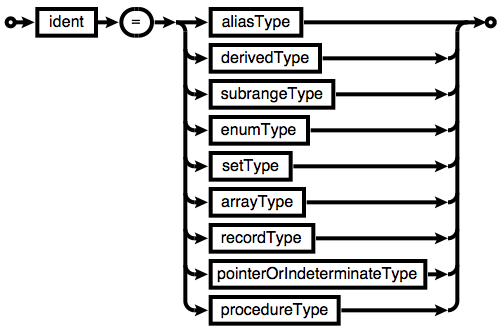
\includegraphics[scale=0.75]{typeDeclaration.png}

\paragraph{\sourcecaption{Pointer or Indeterminate Type}}~

\noindent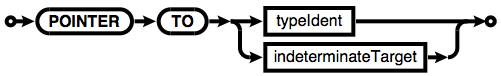
\includegraphics[scale=0.75]{pointerOrIndeterminateType.png}

\paragraph{\sourcecaption{Indeterminate Target}}~

\noindent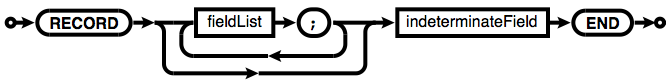
\includegraphics[scale=0.75]{indeterminateTarget.png}

\paragraph{\sourcecaption{Indeterminate Field}}~

\noindent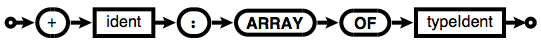
\includegraphics[scale=0.75]{indeterminateField.png}

\newpage

% *****************************************************************************
% D  e  f  i  n  i  t  i  o  n  s
% *****************************************************************************
\printglossary[title=Definitions, toctitle=Definitions]


% *****************************************************************************
% R  e  f  e  r  e  n  c  e  s
% *****************************************************************************
\bibliographystyle{plain}
\bibliography{Indeterminate-Records}
\end{document}

%%% E N D   O F   D O C U M E N T
